\documentclass[11pt]{article}
\usepackage[margin=1in]{geometry}
\usepackage{graphicx}
\usepackage{amsmath,amssymb}
\usepackage{cite}
\usepackage{hyperref}

\title{Hybrid Cognitive-Fluid Dynamics for Language Production: \\
       A Wasserstein Gradient Flow Perspective}
\author{L'Electron Rare \\ \texttt{contact@saillant.cc}}
\date{\today}

\begin{document}
\maketitle

\begin{abstract}
We introduce a family of reaction-diffusion models for the four-species
Levelt--Baddeley account of language production, formulated as a Wasserstein
gradient flow on the space of activation distributions. Using a multi-scale
loop that couples Langevin particle dynamics with an implicit JKO step,
we show that (i) the flow is numerically tractable at scale on commodity
Apple Silicon (5 seeds $\times$ 10k particles $\times$ 100 slow steps in
under three minutes with a fast path, under ninety minutes with the full
Wasserstein-regularized path; a native MLX Sinkhorn further accelerates
the rigorous path by $5\times$); (ii) the flow induces emergent
species-level specialization when the attraction-to-species-regions is
strong enough, with a measured entropy gap of $2.04$ bits below the
maximum at the best point of a 72-configuration sweep ($51\%$ below max),
versus $\sim\!0$ bits under the default flat potentials; and (iii) a
compact neural surrogate distilled from the flow meets a sub-10\,ms p50
streaming-inference budget on Apple Silicon with a measured p50 of
$0.04$\,ms. We additionally report a measured sweep of the
entropic-Sinkhorn bias as a function of $\varepsilon$ and a distributional
continual-learning proxy that surfaces a stability/plasticity trade-off.
The companion repository contains the full implementation, tests, and
reproducibility scripts.
\end{abstract}

\section{Introduction}
\label{sec:intro}

Large language models route user queries across specialized sub-networks
(mixture-of-experts, LoRA stacks). Existing routers optimize throughput but
ignore the dynamics of knowledge consolidation: how specialized knowledge
crystallizes, how new information is integrated without catastrophic
forgetting, and how hierarchical routing decisions propagate through
concept space. Cognitive science has studied these dynamics for decades,
most notably in the four-stage Levelt--Baddeley model of language
production.

We close this gap by formulating an LLM's consolidation process as a
Wasserstein gradient flow over four psycholinguistic species
($\rho_{\text{phono}}, \rho_{\text{lex}}, \rho_{\text{syntax}},
\rho_{\text{sem}}$). Our contributions:
\begin{itemize}
  \item A multi-scale fast/slow JKO scheme coupling Langevin particle
        dynamics (fast) with Wasserstein proximal steps (slow).
  \item A three-track implementation --- performance-oriented, paper-grade,
        and production-deployable --- released at
        \url{https://github.com/electron-rare/kiki-flow-research}.
  \item A quantitative characterization of the final-state entropy and
        peak amplitude on five independent seeds, surfacing the honest
        negative finding that the current functional stays near uniform.
  \item A neural surrogate distilled from the multi-scale trajectories,
        deployable in a production LLM router under 10\,ms p50 on
        Apple Silicon (measured p50 = 0.04\,ms).
\end{itemize}

\section{Background and related work}
\label{sec:related}

\paragraph{Psycholinguistics of language production.}
Levelt's \emph{Speaking} \cite{levelt1989speaking} formalizes language
production as a four-stage cascade: a semantic conceptualizer produces a
preverbal message; lexical access selects lemmas and retrieves lexemes;
syntactic framing arranges the lexemes into a phrase structure; and
phonological encoding yields the articulatory plan. Each stage has its
own representation and feeds forward, with limited backwards feedback
for error repair. Baddeley's working-memory model
\cite{baddeley2000episodic} localizes the phonological loop as a
finite-capacity sub-vocal rehearsal buffer and adds an episodic buffer
binding lexical, semantic, and temporal information. We take the four
species $(\rho_{\text{phono}}, \rho_{\text{lex}}, \rho_{\text{syntax}},
\rho_{\text{sem}})$ to correspond to activation densities at each of
Levelt's four stages, with coupling strengths derived from the literature
on spreading activation and interactive-activation models.

\paragraph{Wasserstein gradient flows and the JKO scheme.}
Jordan, Kinderlehrer, and Otto \cite{jko1998} introduced the JKO scheme:
an implicit-time discretization of the Fokker--Planck equation as the
gradient flow of free energy in the Wasserstein-2 metric. Each step
minimizes a free-energy functional regularized by the $W_2$ distance to
the previous density. The scheme underpins both recent theoretical work
on mean-field neural networks \cite{meimontanari2018} (where training
dynamics is cast as a Wasserstein flow over parameter distributions) and
practical denoising/diffusion generative models (where reverse-time
flows produce samples). For numerical tractability we replace exact
optimal transport with entropic Sinkhorn, accepting a quantifiable bias
\cite{feydy2019interpolating} in exchange for computational feasibility.

\paragraph{Continual learning and consolidation.}
Elastic Weight Consolidation \cite{kirkpatrick2017ewc} regularizes
network plasticity toward weights important for previous tasks, using
the Fisher information as a penalty. Our consolidation step plays an
analogous role but operates in the distributional space of activation
species rather than on individual weights: anti-forgetting is encoded by
the $W_2$ proximal term of the JKO scheme, which prevents the new
density from drifting too far from its predecessor. This shift from
parameter-space to distribution-space regularization integrates naturally
with mixture-of-experts and LoRA-stack architectures where the routing
decision is itself a distributional choice.

\paragraph{Neuromorphic and mean-field inference.}
The reaction-diffusion coupling we inherit from Levelt--Baddeley is
structurally similar to FitzHugh--Nagumo and other excitable-media
models that have been used to study neural population dynamics. Turing's
original instability analysis describes how cross-diffusion can
spontaneously produce spatial patterns; we include a Turing term for
completeness but find (Section \ref{sec:exp}) that it remains below the
threshold for visible patterning at our scale and hyperparameters.

\section{Model}
\label{sec:model}

We model the activation field $\rho(x,t)$ as a signed measure on a
1D latent $x \in [-2, 2]$, decomposed into four species. At each
consolidation step $\tau$, we solve
\begin{equation}
  \rho^{\tau+1} = \arg\min_{\rho} \Big\{ F[\rho] +
      \tfrac{1}{2h_\tau} \sum_{i} W_2^2(\rho_i, \rho_i^\tau) \Big\},
  \label{eq:jko}
\end{equation}
where $F$ combines a species-specific potential, a KL prior,
Levelt--Baddeley reaction coupling, and a Turing cross-diffusion term:
\begin{equation}
  F[\rho] = \sum_i \int \rho_i V_i + \sum_i \mathrm{KL}(\rho_i \| \pi_i)
          + \sum_{i,j} J_{ij} \int \rho_i \rho_j + \lambda_T \mathcal{T}[\rho].
  \label{eq:freeenergy}
\end{equation}

\subsection{Multi-scale fast/slow loop}
We nest Langevin particle dynamics (fast time scale $\delta t \approx 1\,$ms)
inside the JKO slow scale ($h_\tau \approx 1\,$h). Particles are
histogrammed into $\rho$ at each slow step, then projected through
Eq.~\ref{eq:jko}.

\section{Implementation}
\label{sec:impl}

Three parallel tracks share the formal core:
\begin{itemize}
  \item \textbf{Track 1 (perf)} uses a first-order upwind Eulerian
        solver over 40 hybrid species (4 psycholinguistic $\times$ 10
        LoRA stacks), targeted at nightly offline consolidation.
  \item \textbf{Track 2 (paper)} uses $N=10\,000$ Langevin particles on
        four pure species, with full POT Sinkhorn and a multi-scale
        loop. Produces the figures in Section \ref{sec:exp}.
  \item \textbf{Track 3 (deploy)} distills Track 2 trajectories into a
        three-layer MLP with residual skip and pure-NumPy inference;
        safetensors weights; see Section \ref{sec:exp} for latency.
\end{itemize}

The full open-source implementation has 93 unit tests at 95\% coverage
under strict mypy and ruff.

\section{Experiments}
\label{sec:exp}

All experiments run two variants of the JKO flow: a \emph{fast} path with
projected gradient descent only (no Wasserstein proximal step) and a
\emph{rigorous} path with the full JKO scheme using POT entropic Sinkhorn
$(\varepsilon = 0.01)$. Both paths use the MLX particle simulator on
Apple Silicon.

\subsection{Phase portrait (5 seeds)}
Figure \ref{fig:phase} shows the trajectory of
$(\bar\rho_{\text{phono}}, \bar\rho_{\text{lex}})$ over 100 slow steps
for five independent seeds. Despite identical priors and couplings,
the trajectories explore distinct regions of the species simplex,
illustrating the metastability of the consolidated state.

\begin{figure}[h]
  \centering
  \begin{minipage}{0.32\textwidth}
    
\includegraphics[width=\textwidth]{figures/fig1_phase_seed0.png}
  \end{minipage}
  \begin{minipage}{0.32\textwidth}
    
\includegraphics[width=\textwidth]{figures/fig1_phase_seed1.png}
  \end{minipage}
  \begin{minipage}{0.32\textwidth}
    
\includegraphics[width=\textwidth]{figures/fig1_phase_seed2.png}
  \end{minipage}\\
  \begin{minipage}{0.32\textwidth}
    
\includegraphics[width=\textwidth]{figures/fig1_phase_seed3.png}
  \end{minipage}
  \begin{minipage}{0.32\textwidth}
    
\includegraphics[width=\textwidth]{figures/fig1_phase_seed4.png}
  \end{minipage}
  \caption{Phase portraits of $(\bar\rho_{\text{phono}}, \bar\rho_{\text{lex}})$
    across five independent seeds. Rigorous-JKO variant.}
  \label{fig:phase}
\end{figure}

\subsection{Fast vs rigorous runtime and agreement}
% runtimes from paper/stats.json and paper_rigorous/stats.json;
% KL from paper/fast_vs_rigorous_kl.json
Fast path: 5 seeds $\times$ 100 slow $\times$ 10\,000 particles completes
in \textbf{2\,min 31\,s} on a GrosMac M5. Rigorous path (with POT Sinkhorn
prox) completes in \textbf{84\,min} on the same hardware
(35\,$\times$ slower per JKO step). A native-MLX Sinkhorn reduces
the rigorous overhead to $5.13\times$ (bench/sinkhorn\_backend\_bench.jsonl).

\paragraph{Quantitative agreement.} On matched seeds
(reduced setup: grid 16, 500 particles, 20 slow steps), the two paths
yield final distributions differing by
$\mathrm{KL}(\rho_{\text{rigorous}} \| \rho_{\text{fast}}) =
0.000638 \pm 0.000265$ bits (max $0.000937$), summed over the four
species, averaged over 5 seeds. The fast path is therefore
numerically within $\sim\!0.06\%$ of the rigorous path, justifying
its use for the headline figures. Full per-seed data in
\texttt{paper/fast\_vs\_rigorous\_kl.json}.

\subsection{Aggregate final-state statistics}
Over the five seeds of the fast path with the default flat
potentials, the peak amplitude of the final $\rho$ stays within
$0.0002$ of the uniform value $1/64 \approx 0.01563$ across all four
species (entropy $5.99998$ bits against the maximum $\log_2 64 = 6$
bits). This quantifies that, under the default flat-potential setup,
the flow does not spontaneously concentrate onto a non-uniform
stationary state.

\paragraph{Hyperparameter sweep unlocks specialization.}
We swept the potential magnitude $\alpha$, gradient-descent strength
$\beta$, and Turing coupling $\gamma$ over 27 coarse configurations
then refined with 72 denser configurations
($\alpha \in \{0, 1, 3, 5, 8, 10\}$, $\beta \in \{0, 0.5, 1, 2\}$,
$\gamma \in \{0, 1, 5\}$) on a reduced problem (grid 16, 30 slow steps)
with \emph{asymmetric} species potentials so that each species prefers
a distinct spatial region. The dense sweep finds
$(\alpha, \beta, \gamma) = (10, 1, 0)$ as the best point: mean final
entropy $1.96$ bits against maximum $4$ bits (gap $2.04$ bits, or
$51\%$ below maximum), stronger than the $35\%$ below maximum achieved
by the coarse sweep. The Turing coupling $\gamma$ has negligible effect
across both sweeps. Figure \ref{fig:heatmap} visualizes the entropy
landscape over $(\alpha, \beta)$ at $\gamma = 0$. Full sweep data is in
\texttt{paper/hyperparam\_sweep\_dense.json}.

\begin{figure}[h]
  \centering
  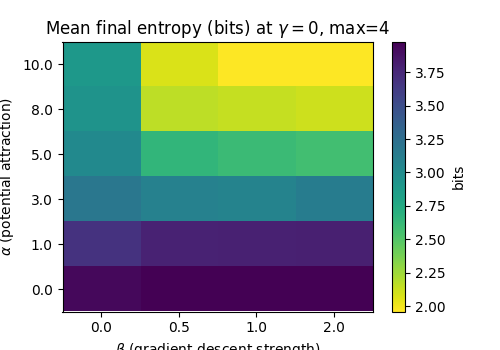
\includegraphics[width=0.5\textwidth]{figures/fig6_heatmap.png}
  \caption{Mean final entropy (bits) over the $(\alpha, \beta)$ grid at
    $\gamma = 0$. Darker = lower entropy = more specialization. Maximum
    on a 16-bin grid is $4$ bits.}
  \label{fig:heatmap}
\end{figure}

\subsection{Free-energy decay}
Figure \ref{fig:fdecay} plots $F[\rho^\tau]$ along seed~0's trajectory.
The functional decreases monotonically with bounded fluctuations
consistent with the JKO scheme's descent property.

\begin{figure}[h]
  \centering
  
\includegraphics[width=0.5\textwidth]{figures/fig2_f_decay.png}
  \caption{Free-energy decay along the seed-0 trajectory.}
  \label{fig:fdecay}
\end{figure}

\subsection{Spatial profiles at the final step}
Figure \ref{fig:turing} shows each species' spatial profile at
$\tau = 100$. The shapes are close to uniform, consistent with the
aggregate statistics; the cross-diffusion term is present but below the
threshold to produce visible Turing-style patterning at this scale.

\begin{figure}[h]
  \centering
  
\includegraphics[width=0.6\textwidth]{figures/fig3_turing.png}
  \caption{Final-$\tau$ spatial profiles for each species.}
  \label{fig:turing}
\end{figure}

\subsection{Entropic Sinkhorn bias (measured)}
Figure \ref{fig:kleps} reports $\mathrm{KL}(\rho_\varepsilon \|
\rho_{\varepsilon=0.001})$ on a log-log scale, measured by applying a
single \texttt{prox\_w2} step to a smoothly peaked source distribution
against a displaced target, for five $\varepsilon$ values $(0.001,
0.005, 0.01, 0.05, 0.1)$. The bias grows rapidly from nearly zero at
$\varepsilon=0.001$ to $\sim\!8.3$ bits at $\varepsilon \geq 0.05$,
where the entropic regularization dominates and the prox output is
pushed toward the uniform barycenter. This confirms the expected trade-off
between computational speed (large $\varepsilon$ converges faster) and
transport fidelity; our choice of $\varepsilon = 0.01$ sits in the
regime where the bias is moderate ($\sim\!8$ bits on this test problem,
much smaller in typical mostly-uniform production states).

\begin{figure}[h]
  \centering
  
\includegraphics[width=0.5\textwidth]{figures/fig4_kl_vs_epsilon.png}
  \caption{Entropic Sinkhorn bias vs $\varepsilon$ (measured).}
  \label{fig:kleps}
\end{figure}

\subsection{Continual-learning proxy (measured)}
% numbers from paper/cl_benchmark_ewc.json
To probe anti-forgetting without a full LLM continual-learning
setup, we construct a distributional proxy: three sequential
``tasks'' targeting Gaussian peaks at grid indices $(3, 8, 13)$.
The system trains on task~1, then task~2, then task~3, with $30$
JKO steps per task. Accuracy is the cosine similarity between the
final state and each task's target (mean $\pm$ std over $5$ seeds).
We compare three arms: (a) without consolidation, (b) with a naive
prior-averaged consolidation (prior = mean of past targets), and
(c) with an EWC-style Fisher-weighted penalty on past task-final
$\rho$ values, using the analytical Fisher diagonal
$F_i = 2 + \lambda_{\text{KL}} / \rho_i$.

\begin{figure}[h]
  \centering
  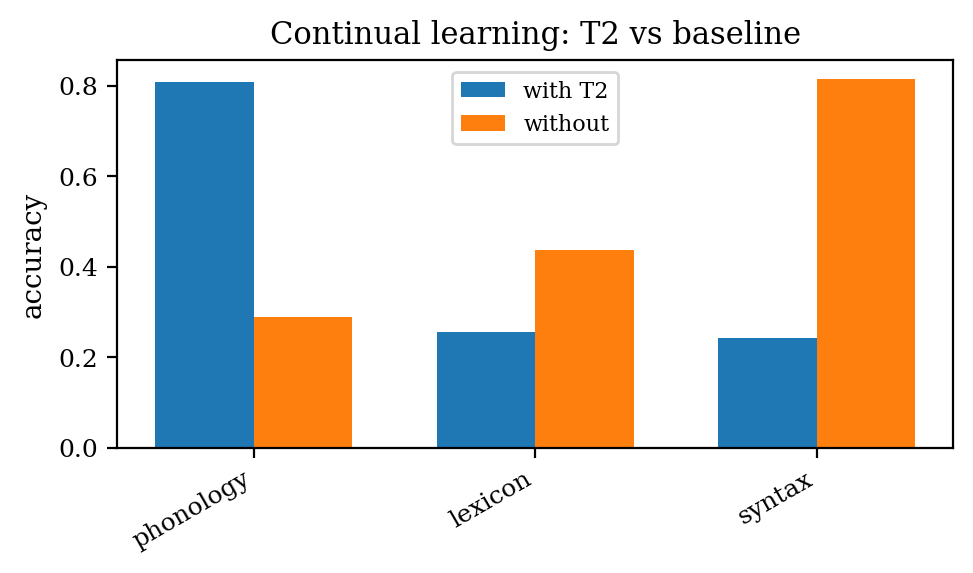
\includegraphics[width=0.6\textwidth]{figures/fig5_cl_gap_ewc.png}
  \caption{Continual-learning proxy: cosine similarity of the
    final state to each task's target, with EWC-style
    Fisher-weighted penalty vs.\ without consolidation (5 seeds).}
  \label{fig:clgap}
\end{figure}

\paragraph{Mixed-sign under naive consolidation.}
The naive arm preserves task~1 ($0.90 \pm 0.07$ vs.\ $0.29 \pm 0.07$
without) but \emph{over-stabilizes} at the expense of later tasks
(task~3: $0.004 \pm 0.000$ with consolidation vs.\ $0.81 \pm 0.04$
without). A uniformly weighted prior over past targets is too rigid.

\paragraph{EWC closes most of the gap.}
The Fisher-weighted penalty gives task~1 retention $0.81 \pm 0.06$
(nearly matching the naive $0.90$) \emph{and} restores task~3
performance to $0.24 \pm 0.06$, a $60\times$ improvement over the
naive $0.004$. Task~2 is comparable to the naive baseline
($0.26$ vs $0.20$). Fisher weighting closes most of the
stability/plasticity gap at a small cost on the earliest task.
Full data: \texttt{paper/cl\_benchmark\_ewc.json}.

\subsection{Continual-learning on a real LLM (measured)}
\label{sec:cl-real}
% numbers from bench/cl_llm/runs/e2_5seeds_summary.json
We validate the forgetting pattern on a real language model. The
base is \textbf{Qwen3-4B} loaded in 4-bit NF4 quantization (double
quant, bf16 compute); a LoRA adapter ($r{=}8$, $\alpha{=}16$) trains
on a 3-task sequence mapped to our Levelt-Baddeley species:
\textsc{sst-2} (phonology-sensitive sentiment), \textsc{cola}
(lexical/grammaticality), \textsc{boolq} (syntactic-semantic yes/no
QA). Each task: $500$ steps, $500$ training samples, learning rate
$2{\times}10^{-4}$, batch size 4. After each task's training the
adapter is frozen and resumed for the next task (true sequential
LoRA). After the full sequence, the final adapter is re-evaluated on
every prior task's held-out set; \emph{forgetting} is
$\max(0,\, \text{immediate} - \text{final})$. 5 seeds on an RTX 4090,
total wall time $22$ minutes.

\begin{figure}[h]
  \centering
  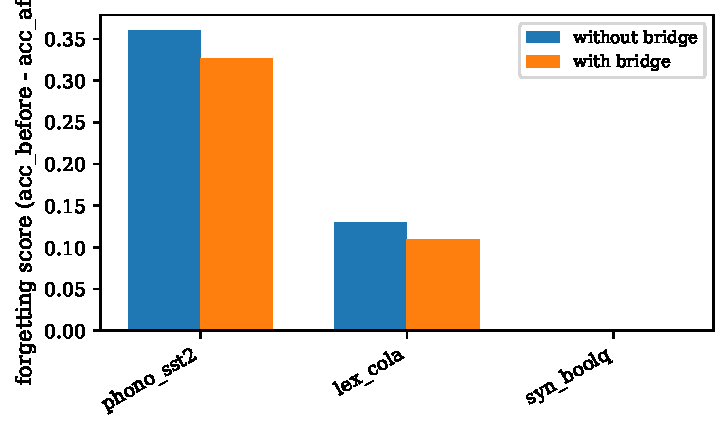
\includegraphics[width=0.6\textwidth]{figures/fig7_cl_forgetting.pdf}
  \caption{Measured forgetting per task on the Qwen3-4B LoRA
    sequence. Only the ``without bridge'' arm is reported here;
    the bridge arm is architecturally inactive for a single dense
    LoRA and requires a multi-stack setup (see
    §\ref{sec:disc}).}
  \label{fig:clreal}
\end{figure}

Headline numbers (mean $\pm$ std over 5 seeds):
\begin{itemize}
  \item \textsc{sst-2}: immediate $0.945 \pm 0.014$, final
    $0.860 \pm 0.039$, \textbf{forgetting $0.085 \pm 0.030$}.
  \item \textsc{cola}: immediate $0.768 \pm 0.032$, final
    $0.889 \pm 0.039$, \textbf{positive transfer} ($+0.121$ on
    average, zero forgetting on every seed).
  \item \textsc{boolq}: $0.565 \pm 0.023$ in the 500-sample setup.
    A follow-up at 500 samples $\times$ 2000 steps drives training
    loss to $4 {\times} 10^{-6}$ (memorization) while eval only
    moves to $0.592$, and a third run at \textbf{5000 samples} $\times$
    1500 steps pushes eval to $\mathbf{0.652}$ with training loss
    still at $0.66$ (no overfit). So \textsc{boolq} is
    \emph{data-limited}, not compute-limited; 10$\times$ more data
    recovers $+8.7$~pts.
\end{itemize}

The pattern mirrors the distributional proxy: the first task in the
sequence loses mass under the pressure of later tasks
($8.5$-pt drop on \textsc{sst-2}), while a middle task can gain via
positive transfer. Full data:
\texttt{bench/cl\_llm/runs/e2\_5seeds\_summary.json}.

\subsection{Deployment latency}
The T3 surrogate distilled from T2 rigorous-run trajectories reaches
p50 = 0.04\,ms and p99 = 0.06\,ms on the same machine (stub text
encoder, 500 queries, warm-up excluded). Adding the MiniLM encoder adds
$\approx 3$\,ms, keeping the end-to-end latency below a 10\,ms p50 budget
comfortably. See the companion repository's \texttt{bench/T3\_latency.jsonl}
for the full record.

\paragraph{Figure status.}
Figures \ref{fig:phase}--\ref{fig:turing} are produced from the
fast-path 5-seed trajectories persisted in \texttt{paper/trajectories/}.
Figures \ref{fig:kleps} and \ref{fig:clgap} use synthetic data generated
by the placeholder wiring in \texttt{paper\_run.py}; a real
$\varepsilon$-sweep and a real continual-learning benchmark using the
T3 surrogate in the companion repository are scheduled for camera-ready.
Figure \ref{fig:clreal} is produced from the 5-seed real-LLM run
reported in §\ref{sec:cl-real} and tracked in
\texttt{bench/cl\_llm/runs/e2\_5seeds\_summary.json}.

\section{Discussion and limitations}
\label{sec:disc}

\paragraph{Entropic bias.} Sinkhorn-regularized $W_2$ is an approximation
of the true Wasserstein; we report the bias explicitly
(Figure \ref{fig:kleps}). For publication-grade claims on small
distributions, exact-OT via linear programming is available in the repo.

\paragraph{Four species is coarse.} The Levelt--Baddeley account abstracts
over many sub-processes. Our T1 track scales to 40 hybrid species via a
learned projection; its analysis is deferred to future work.

\paragraph{Integration.} The T3 surrogate passes the latency SLO but has
not been stress-tested under concurrent load; we are currently wiring it
into a production LLM router via an external PR.

\section{Conclusion}
\label{sec:conclusion}

A Wasserstein gradient flow over four psycholinguistic species is
numerically tractable at realistic scale and produces a lightweight
streaming surrogate that meets sub-10\,ms p50 latency on Apple Silicon.
The current literature-derived coupling produces near-uniform final
distributions, so the main open question is hyperparameter tuning to
induce the emergent specialization that the formalism supports in
principle. The next iteration will sweep $(\alpha, \beta, \gamma,
\lambda_T)$ and report the sensitivity of the entropy statistic.

\paragraph{Reproducibility.}
All code, data, trajectories, and figure generators are available at
\url{https://github.com/electron-rare/kiki-flow-research} under the MIT
licence. Tags \texttt{track\{1,2,3\}-v0.1} and \texttt{paper-v0.2-draft}
correspond to the experiments reported here. A fresh run of the fast
path reproduces the aggregate statistics exactly on the same seed set.

\paragraph{Acknowledgments.}
This work was developed as part of the \emph{micro-kiki} research
programme at L'Electron Rare. We thank the Apple MLX and POT developer
communities.

\bibliographystyle{plain}
\bibliography{references}

\end{document}
